Cells are organised in different subcellular structures,
which is more complex in the Eukarya compared to the Bacteria and Archaea.
Different eukaryotic cellular structures include:
the nucleus,
plasma membrane,
cell wall,
different types of organelles,
and the endoplasmic reticulum.
By separating the cell in subcellular compartments, 
there can be a physical separation of different functions.
For example,
Mitochondria focus on the production of energy,
chloroplasts capture electromagnetic energy  by storing it into carbon based molecules,
and the nucleus contains the genetic information.
In addition, each compartment has its own local environment and conditions,
evolutionary tuned to the function it has to perform.
Animal and plant subcellular compartments are the most studied structures (Fig. \ref{fig:eukaryotic_cell_structure}).
While they both contain 
a nucleus, 
cytoplasm,
plasma membrane, 
endoplasmic reticulum,
and mitochondria,
there are some striking differences as well. 
The centrosome and lysosomes are unique organelles form animal cells. 
Plant cells on the other hand have a 
cell wall, 
a large central vacuole, 
chloroplasts and other specialized plastids
(\cite{boundless_biology_eukaryotic}).

~\begin{figure}[h!]
  \centering
  ~\begin{subfigure}[b]{0.45\linewidth}
    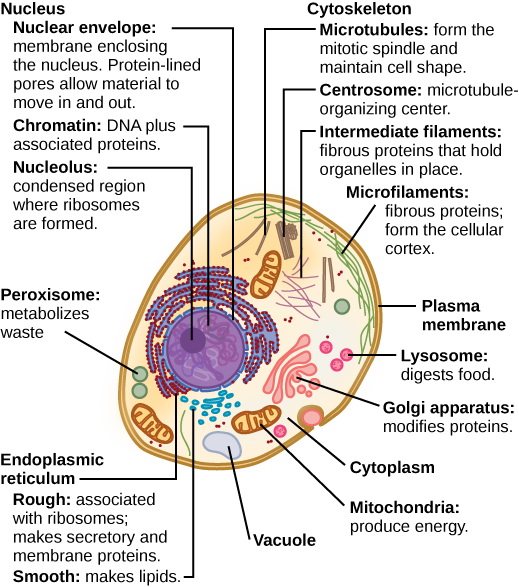
\includegraphics[width=\linewidth]
	{./literature_review/subcellular_location/protein_localization/img/animal_cell_structure.png}
  \caption{Animal cell}
  ~\end{subfigure}
\hfill
  ~\begin{subfigure}[b]{0.48\linewidth}
    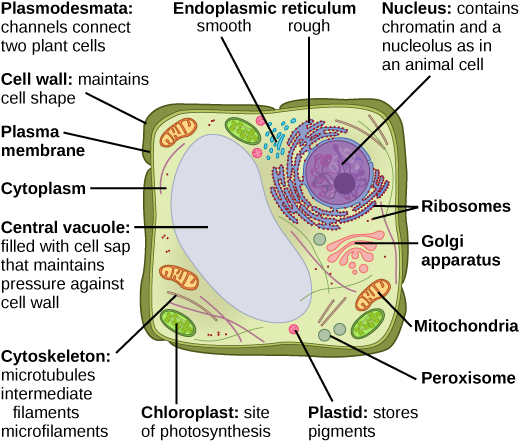
\includegraphics[width=\linewidth]
	{./literature_review/subcellular_location/protein_localization/img/plant_cell_structure.png}
  \caption{Plant cell}
  ~\end{subfigure}
  \caption{
\textbf{The eukaryotic cell structure.} 
Eukaryotic cells are subdivided in different subcellular compartments.
Shown are the animal and plant cell.
(from \cite{boundless_biology_eukaryotic}).
}
  \label{fig:eukaryotic_cell_structure}
~\end{figure}

The prokaryotic cell structure of Bacteria and Archaea is less complex than the eukaryotic structure.
Similarly, the plasmamembrane contains the cytoplasm.
Unlike eukaryotes, prokaryotic genetic DNA is not encapsulated by a nucleus,
but localised in a region called the nucleoid.
Prokaryotic cells are much smaller their eukaryotic counterparts,
and they lack organelles
(\cite{boundless_biology_prokaryotic}).
Bacteria can be divided into two major groups based on their Gram stain reaction
(Fig. \ref{fig:prokaryotic_cell_structure}).
Gram-negative cells have a cell wall that is made out of two layers:
a small peptidoglycan layer, 
and outer membrane containing a lipid bilayer and polysacharides.
The region between the inner and outer membrane is called the periplasm.
Gram-positive Bacteria have a thick mono-layer cell wall, mostly made out of peptidoglycan,
but no outer membrane
(\cite{madigan2015}).


~\begin{figure}[h!]
  \centering
  ~\begin{subfigure}[b]{\linewidth}
    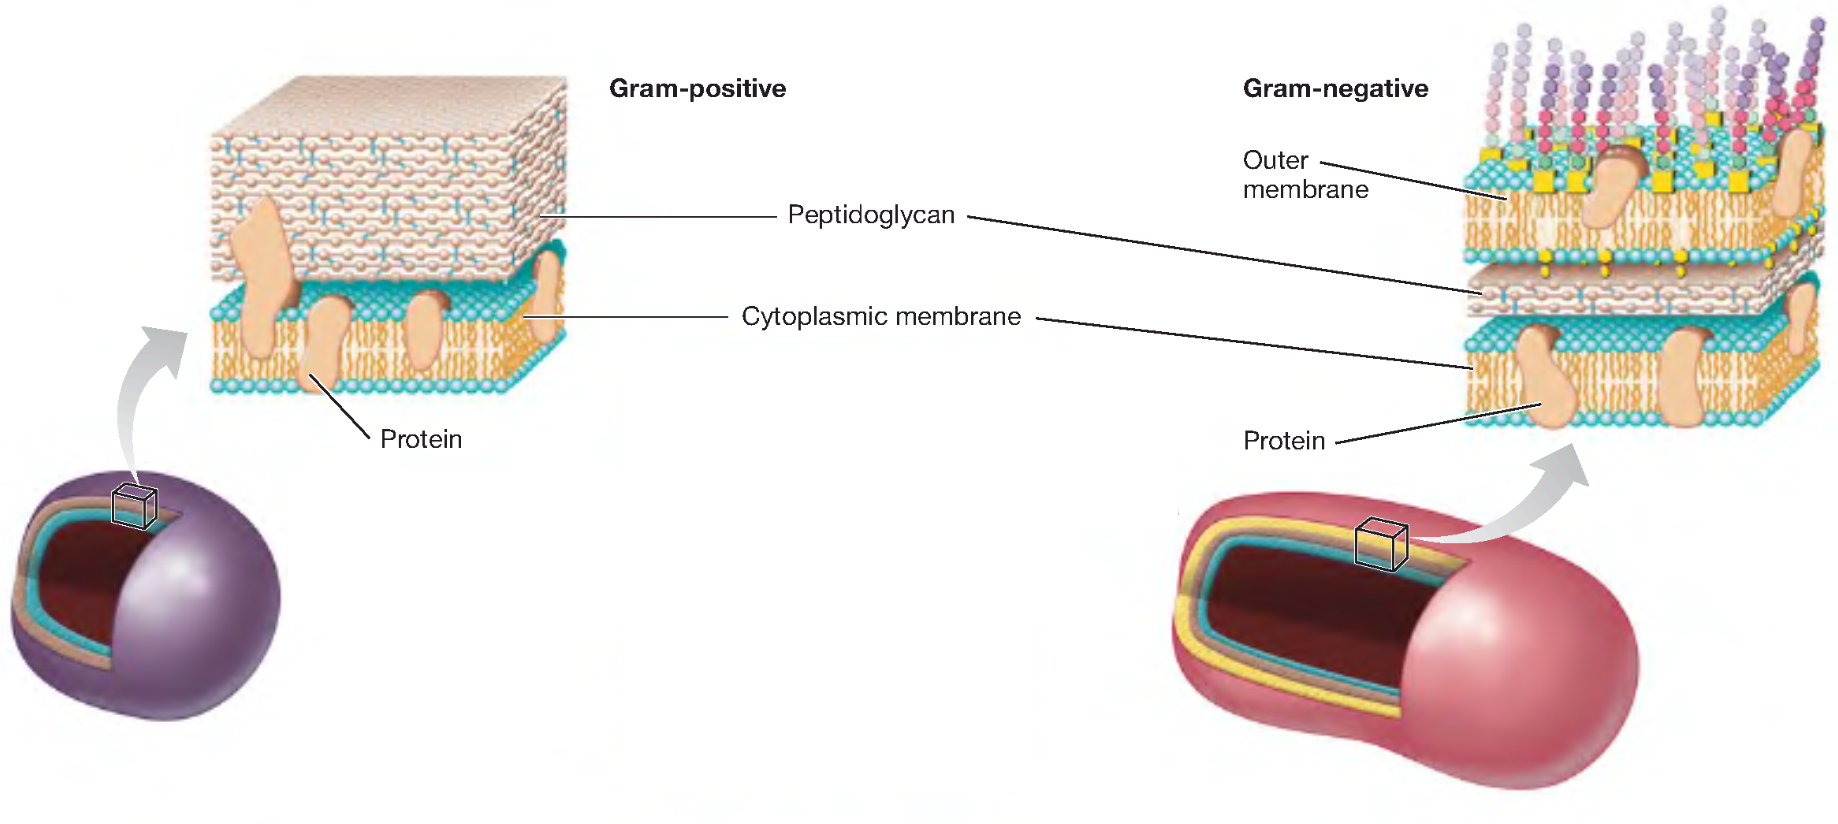
\includegraphics[width=\linewidth]
	{./literature_review/subcellular_location/protein_localization/img/gram_pos_vs_neg.png}
  ~\end{subfigure}
  \caption{
\textbf{The prokaryotic cell structure of gram positive and gram negative Bacteria.} 
(adapted from \cite{madigan2015}).
}
  \label{fig:prokaryotic_cell_structure}
~\end{figure}


